\chapter{Experiments and Improvements}\label{experiments_and_improvements}

In order to enhance the proposed model, we employed different strategies for finding improvements: \begin{itemize}
	\item Removing some input features to improve the robustness of the model.
	\item Testing smaller, more data-efficient networks to optimize the current architecture.
	\item Experimenting with more powerful architectures, such as Transformers, which have demonstrated remarkable success in natural language processing (NLP).
	\item Extending the model by introducing an additional module for handling other musical elements: dynamics. \end{itemize}
	
In subsequent experiments we stepped out from the full Transformer for attention mechanism only. We wanted to check whether access to the entire tensor sequence is beneficial for the transcription task. However, in the preliminary experiments combinations of self-attention mechanism with other components didn't perform as well as the base model nor Transformer-based ones, and the self-attention-based models have been excluded from the study.
	
Let us present results of these experiments.

\section{Ablation Studies} \label{ablation_studies}

To validate the assumptions presented in Section \ref{robustness_analysis}, we conducted ablation studies by training models that utilized only a restricted set of input features. Specifically, the following configurations were employed: \begin{itemize}
	\item The \textbf{hand part} model was trained only on note pitches and onsets.
	\item The \textbf{key signature} model was trained only on note pitches and onsets.
	\item The \textbf{time signature} model was trained using only note onsets.
\end{itemize}

As a result, all models became invulnerable to transformations described in the Section \ref{perturbations}. This section evaluates the impact of such feature reduction on model performance.

Each model was evaluated using two metrics:
\begin{itemize} \item Model-specific $F_1$ scores. \item The MV2H metric, with restricted models replacing their corresponding original components. \end{itemize}

All evaluations were conducted on the test subset of the dataset, with both base and restricted models trained exclusively on the training set. For a fair comparison, the model with the best validation $F_1$ score across 50 epochs was selected for each ablation study.

\subsection{Beat Tracking} \label{beat_tracking}

The authors of the original paper provided ablation studies for the beat-tracking model, analyzing how the omission of features and data augmentation influenced its performance. The results of these analyses are summarized in Tables \ref{beat_tracking_feature_omission} and \ref{beat_tracking_data_augmentation}.

\begin{table}[ht!]
\centering
\begin{tabular}{cccc}
    \textbf{Feature omitted} & Precision & Recall  & $F_1$ score   \\\hline
    Pitch                    & $0.904$   & $0.937$ & $0.906$       \\
    Onset                    & $0.846$   & $0.728$ & $0.764$       \\
    Duration                 & $0.895$   & $0.931$ & $0.901$       \\
    Velocity                 & $0.895$   & $0.939$ & $0.906$       \\
    Use all features         & $0.912$   & $0.943$ & ${\bf 0.913}$ \\
\end{tabular}

\caption[Feature omission study.]{Feature omission study \cite{Liu2022}.}
\label{beat_tracking_feature_omission}
\end{table}

Not surprisingly, note onsets are the most important feature used by the beat-tracking model. While neglecting other features doesn't hardly impact the model, still feature omission results in a slight quality degradation.

Velocity may carry some information about beats as they tend to occur along with heavier notes \cite{Liu2022}. Harmonic structure inferred by pitch may also transfer such information, for example it is quite common to play chords at the beginning of a measure. Note durations may also offer hints about the underlying meter.

\begin{table}[ht!]
\centering
\begin{tabular}{cccc}
    \textbf{Augmentation method omitted} & Precision & Recall  & $F_1$ score      \\\hline
    Pitch shift                          & $0.920$   & $0.920$ & $0.906$          \\
    Tempo change                         & $0.918$   & $0.895$ & $0.897$          \\
    Note removal                         & $0.915$   & $0.909$ & $0.904$          \\
    Extra note insertion                 & $0.912$   & $0.943$ & $0.913$          \\
    Use all methods                      & $0.929$   & $0.937$ & $\mathbf{0.922}$ \\
    No data augmentation                 & $0.897$   & $0.952$ & $0.909$
\end{tabular}

\caption[Ablation study for data augmentation.]{Ablation study for data augmentation \cite{Liu2022}.}
\label{beat_tracking_data_augmentation}
\end{table}

\subsection{Hand Part Model}

A variant of the hand part model was trained without using note durations or velocities. As the hand part assignment influences only the voice separation subscale of the MV2H metric, other submetrics were excluded from the evaluation.

\begin{table}[ht!]
\centering
\begin{tabular}{ccc}
    \textbf{Metric}  & \textbf{Standard} & \textbf{Restricted} \\\hline
    Accuracy         & $0.956$           & $0.949$                \\
    Precision        & $0.851$           & $0.843$                \\
    Recall           & $0.848$           & $0.845$                \\
    $F_1$-score      & $0.842$           & $0.840$                \\
    Voice separation & $0.852$           & $0.818$                \\
\end{tabular}

\caption[Ablation study for the hand part model.]{Ablation study for the hand part model.}
\label{hand_part_ablation}
\end{table}

The results (Table \ref{hand_part_ablation}) show comparable performance between the restricted and original models across all metrics. This indicates that velocity provides marginal, if any, additional information for hand part assignment. These findings align with the observations in Section \ref{results}, where velocity had a limited influence on model predictions.

\subsection{Key Signature Model}

The restricted key signature model, trained using only note pitches and onsets, achieved performance similar to the original model.

\begin{table}[ht!]
\centering
\begin{tabular}{cccc}
    \textbf{Type}             & \textbf{Metric} & \textbf{Standard} & \textbf{Restricted} \\\hline
    \multirow{3}{*}{Macro}    & Precision       & $\mathbf{0.812}$  & $0.807$             \\
    & Recall          & $\mathbf{0.789}$  & $0.788$             \\
    & $F_1$ score     & $\mathbf{0.787}$  & $0.786$             \\\hline
    \multirow{3}{*}{Weighted} & Precision       & $\mathbf{0.924}$  & $\mathbf{0.924}$    \\
    & Recall          & $0.898$           & $\mathbf{0.904}$    \\
    & $F_1$ score     & $0.896$           & $\mathbf{0.900}$    \\\hline
    \multicolumn{2}{c}{Harmony} & $\mathbf{0.972}$ & $\mathbf{0.972}$ \\
\end{tabular}

\caption[Ablation study for the key signature model.]{Ablation study for the key signature model.}
\label{key_signature_ablation}
\end{table}

Table \ref{key_signature_ablation} shows the results with included the harmony MV2H subscale. Let us remind that weighted metric results are calculated independently, and weighted by the number of true labels of each class, while macro metrics are unweighted.

The observed differences fall within the expected range of model stochasticity. The result agrees also with the negligible influence of other factors to the final model decision on key signature, described in Section \ref{results}.

\subsection{Time Signature Model}

A restricted time signature model, trained solely on note onsets, outperformed the original convolutional network classifier in terms of $F_1$ scores.

\begin{table}[ht!]
\centering
\begin{tabular}{ccc}
    \textbf{Metric}  & \textbf{Standard} & \textbf{Restricted} \\\hline
    Accuracy         & $0.552$           & $0.656$                \\
    Precision        & $0.444$           & $0.571$                \\
    Recall           & $0.333$           & $0.667$                \\
    $F_1$ score      & $0.381$           & $0.615$
\end{tabular}

\caption[Ablation study for the time signature model.]{Ablation study for the time signature model.}
\label{time_signature_ablation}
\end{table}

Interestingly, as the MV2H metric does not directly depend on time signature predictions, substituting the original model with the restricted version had no impact on the overall evaluation. This shows that not only introducing full information to the model is not beneficial, but actually hurts the performance of the model. 

\section{Transformers}

\emph{Transformers} are a class of neural network architectures introduced by Vaswani et al. in the landmark paper \emph{Attention Is All You Need} \cite{Vaswani2017}. Originally developed for natural language processing (NLP), have since become versatile and powerful framework for modeling sequential data across numerous other fields, including image processing \cite{Dosovitskiy2020}, audio generation \cite{Borsos2023} and even symbolic music analysis \cite{Zhu2021}.

\begin{figure}[ht!]
\centering
\begin{tikzpicture}
    \tikzset{block/.style={fill=gray!20, text width=3.5cm, draw=black, thick, text centered, align=center, rounded corners, minimum height=1.5em, minimum width=3.5cm}}
    \tikzset{input/.style={fill=gray!30, text width=3.5cm, draw=black, thick, text centered, rounded corners, minimum height=1.5em, minimum width=3.5cm}}
    \tikzset{operation/.style={draw, circle, thick, minimum size=0.75cm}}
    \tikzset{arrowstyle/.style={-{Latex[length=3mm]}}}

    \node (inputs) at (0, 1.5) {Inputs};
    \node (outputs) at (6, 1.5) {Shifted Outputs};

    \node[input] (input_embed) at (0, 0) {Input Embedding};
    \node[block] (pos_encoding) at (-3, -1.2) {Positional \\ Encoding};
    \node[operation] (add1) at (0, -1.2) {$+$};

    \node[block] (multihead1) at (0, -3.25) {Multi-Head \\ Attention};
    \node[block] (add_norm1) at (0, -4.5) {Add \& Norm};
    \node[block] (ffn1) at (0, -6.25) {Feed \\ Forward};
    \node[block] (add_norm2) at (0, -7.5) {Add \& Norm};

    \draw[rounded corners, thick] (-2.75, -2) rectangle (2.75, -8.25) node[pos=0.5, xshift=-3.1cm] {$N \times \;$};

    \node[input] (output_embed) at (6, 0) {Output Embedding};
    \node[block] (pos_encoding_dec) at (9, -1.2) {Positional \\ Encoding};
    \node[operation] (add2) at (6, -1.2) {$+$};

    \node[block] (masked_mha) at (6, -3.25) {Masked Multi-Head \\ Attention};
    \node[block] (add_norm_dec1) at (6, -4.5) {Add \& Norm};
    \node[block] (mha_dec) at (6, -6.40) {Multi-Head \\ Attention};
    \node[block] (add_norm_dec2) at (6, -7.50) {Add \& Norm};
    \node[block] (ffn2) at (6, -9.25) {Feed \\ Forward};
    \node[block] (add_norm_dec3) at (6, -10.50) {Add \& Norm};

    \draw[rounded corners, thick] (3.25, -2) rectangle (8.75, -11.25) node[pos=0.5, xshift=3.1cm] {$\, \times N$};

    \node[block] (linear) at (6, -12.2) {Linear};
    \node[block] (softmax) at (6, -13.6) {Softmax};
    \node (output_probs) at (6, -15.1) {Output Probabilities};

    \draw[arrowstyle] (inputs.south) -- (input_embed.north);
    \draw[arrowstyle] (input_embed.south) -- (add1.north);
    \draw[arrowstyle] (pos_encoding.east) -- (add1.west);
    \draw[arrowstyle] (add1) -- (multihead1);
    \draw[arrowstyle] (multihead1) -- (add_norm1);
    \draw[arrowstyle] (add_norm1) -- (ffn1);
    \draw[arrowstyle] (ffn1) -- (add_norm2);

    \draw[arrowstyle] (outputs.south) -- (output_embed.north);
    \draw[arrowstyle] (output_embed.south) -- (add2.north);
    \draw[arrowstyle] (pos_encoding_dec.west) -- (add2.east);
    \draw[arrowstyle] (add2) -- (masked_mha);
    \draw[arrowstyle] (masked_mha) -- (add_norm_dec1);
    \draw[arrowstyle] (mha_dec) -- (add_norm_dec2);
    \draw[arrowstyle] (add_norm_dec2) -- (ffn2);
    \draw[arrowstyle] (ffn2) -- (add_norm_dec3);
    \draw[arrowstyle] (add_norm_dec3) -- (linear);
    \draw[arrowstyle] (linear) -- (softmax);
    \draw[arrowstyle] (softmax) -- (output_probs);

    \draw[arrowstyle] (add_norm2.east) -| ++(0.325, 0) |- ++(0, 2.05) -| ($(mha_dec.north) - (1.0, 0.0)$);
    \draw[arrowstyle] (add_norm2.east) -| ++(0.325, 0) |- ++(0, 2.05) -| (mha_dec.north);

    \draw[arrowstyle] (0, -2.25) -| ++(-2.325,0) |- (add_norm1.west);
    \draw[arrowstyle] (0, -5.25) -| ++(-2.325,0) |- (add_norm2.west);

    \draw[arrowstyle] (0, -2.35) -| ++(-1.0,0) -- ($(multihead1.north) - (1.0, 0.0)$);
    \draw[arrowstyle] (0, -2.35) -| ++(1.0,0) -- ($(multihead1.north) + (1.0, 0.0)$);

    \draw[arrowstyle] (6, -2.35) -| ++(-1.0,0) -- ($(masked_mha.north) - (1.0, 0.0)$);
    \draw[arrowstyle] (6, -2.35) -| ++(1.0,0) -- ($(masked_mha.north) + (1.0, 0.0)$);

    \draw[arrowstyle] (add_norm_dec1) -- (6, -5.25) -| ++(1.0,0) -- ($(mha_dec.north) + (1.0, 0.0)$);

    \draw[arrowstyle] (6, -2.25) -| ++(2.325,0) |- (add_norm_dec1.east);
    \draw[arrowstyle] (6, -5.25) -| ++(2.325,0) |- (add_norm_dec2.east);
    \draw[arrowstyle] (6, -8.25) -| ++(2.325,0) |- (add_norm_dec3.east);

\end{tikzpicture}
\caption[The Transformer architecture.]{The Transformer architecture \cite{Vaswani2017}.}
\end{figure}

The key innovation in Transformers is the \emph{self-attention} mechanism, which enables the model to weigh the relevance of each part of an input sequence relative to other parts, regardless of their distance from each other in the sequence. Unlike recurrent neural networks, which process data sequentially and can struggle with long-range dependencies, Transformers use that mechanism to directly model these dependencies in parallel.

As the authors state at the end of the paper \cite{Liu2022}: \begin{quote}Possible next steps include investigating more powerful model architectures such as the Transformer.\end{quote} We analyzed various setups involving Transformer and attention mechanisms, preserving the training and evaluation setup.

\subsection{Vanilla Transformer}

We evaluated a standard Transformer encoder architecture, limited to the encoder block since the transcription task does not involve decoding. As a rule of thumb, we decided to keep the model size comparable to the original network. Different number of embedding sizes have been employed: $128$, $256$ and $512$ dimensions. 

Given that Transformers are designed for sequential discrete data, we applied an additional encoding scheme to discretize note durations and velocities. Features were concatenated prior to positional encoding. Preliminary experiments demonstrated that this approach outperformed the use of continuous floating-point encodings for durations and velocities. The note durations were encoded with the same number of discrete features as onsets, while velocities were reduced to eight discrete categories. The total feature space thus consisted of: \[\underbrace{128}_{\textrm{pitch}}+\underbrace{401}_{\textrm{onset}}+\underbrace{401}_{\textrm{duration}}+\underbrace{8}_{\textrm{velocity}} = 938\]

\begin{figure}[ht!]
\centering
\begin{tabular}{cc}a)
\scalebox{0.8}{
\begin{tikzpicture}
    \tikzset{block/.style={fill=gray!20, text width=3.5cm, draw=black, thick, text centered, align=center, rounded corners, minimum height=1.5em, minimum width=3.5cm}}
    \tikzset{input/.style={fill=gray!30, text width=3.5cm, draw=black, thick, text centered, rounded corners, minimum height=1.5em, minimum width=3.5cm}}
    \tikzset{operation/.style={draw, circle, thick, minimum size=0.75cm}}
    \tikzset{arrowstyle/.style={-{Latex[length=3mm]}}}

    \node (inputs) at (0, 1.5) {Inputs};
    \node[input] (input_embed) at (0, 0) {Input Embedding};
    \node[block] (pos_encoding) at (-3, -1.2) {Positional \\ Encoding};
    \node[operation] (add) at (0, -1.2) {$+$};
    \node[block] (transformer) at (0, -2.7) {Transformer Encoder};
    \node[input] (linear) at (0, -4.2) {Linear};
    \node (output) at (0, -5.7) {Output Probabilities};

    \draw[arrowstyle] (inputs.south) -- (input_embed.north);
    \draw[arrowstyle] (input_embed.south) -- (add.north);
    \draw[arrowstyle] (pos_encoding.east) -- (add.west);
    \draw[arrowstyle] (add) -- (transformer);
    \draw[arrowstyle] (transformer) -- (linear);
    \draw[arrowstyle] (linear) -- (output);

\end{tikzpicture}
} & b)
\scalebox{0.8}{
    \begin{tikzpicture}
    \tikzset{block/.style={fill=gray!20, text width=3.5cm, draw=black, thick, text centered, align=center, rounded corners, minimum height=1.5em, minimum width=3.5cm}}
    \tikzset{input/.style={fill=gray!30, text width=3.5cm, draw=black, thick, text centered, rounded corners, minimum height=1.5em, minimum width=3.5cm}}
    \tikzset{embedding/.style={fill=gray!40, text width=1.5cm, draw=black, thick, text centered, rounded corners, minimum height=1.5em, minimum width=1.5cm}}
    \tikzset{operation/.style={draw, circle, thick, minimum size=0.75cm}}
    \tikzset{arrowstyle/.style={-{Latex[length=3mm]}}}

    \node (pitch) at (-3.0, 1.5) {Pitch};
    \node (onset) at (-1.0, 1.5) {Onset};
    \node (duration) at (1.0, 1.5) {Duration};
    \node (velocity) at (3.0, 1.5) {Velocity};
    \node[embedding] (pitch_embed) at (-3.0, 0) {Embed.};
    \node[embedding] (onset_embed) at (-1.0, 0) {Embed.};
    \node[embedding] (duration_embed) at (1.0, 0) {Embed.};
    \node[embedding] (velocity_embed) at (3.0, 0) {Embed.};
    \node[block] (pos_encoding) at (-3, -2.7) {Positional \\ Encoding};
    \node[operation] (add1) at (0, -1.2) {$+$};
    \node[operation] (add2) at (0, -2.7) {$+$};
    \node[block] (transformer) at (0, -4.2) {Transformer Encoder};
    \node[input] (linear) at (0, -5.7) {Linear};
    \node (output) at (0, -7.2) {Output Probabilities};

    \draw[arrowstyle] (pitch.south) -- (pitch_embed.north);
    \draw[arrowstyle] (onset.south) -- (onset_embed.north);
    \draw[arrowstyle] (duration.south) -- (duration_embed.north);
    \draw[arrowstyle] (velocity.south) -- (velocity_embed.north);
    \draw[arrowstyle] (pitch_embed.south) |- (add1.west);
    \draw[arrowstyle] (onset_embed.south) |- (add1.west);
    \draw[arrowstyle] (duration_embed.south) |- (add1.east);
    \draw[arrowstyle] (velocity_embed.south) |- (add1.east);
    \draw[arrowstyle] (pos_encoding.east) -- (add2.west);
    \draw[arrowstyle] (add1) -- (add2);
    \draw[arrowstyle] (add2) -- (transformer);
    \draw[arrowstyle] (transformer) -- (linear);
    \draw[arrowstyle] (linear) -- (output);

\end{tikzpicture}
}
\end{tabular}
\caption[The Transformer Encoder block.]{The Transformer Encoder block: a) default encoding, b) feature embedding. The second architecture was selected for subsequent experiments. The positional encoding is optional.}
\label{vanilla_transformer_encoder_with_embedding}
\end{figure}

For training, the learning rate was reduced to \num{1e-4}, with a warmup period of 2500 steps. We also tested configurations without positional encoding\footnote{Certain language models have been shown to perform well without explicit positional encodings \cite{Haviv2022}.}. All experiments utilized the default \texttt{pytorch} Transformer encoder implementation.

\subsection{Results}

Overall, Transformer-based models did not match the performance of the base architecture. Positional encoding, in particular, often degraded performance. Even when achieving comparable validation results on specific subtasks, Transformer-based models struggled to generalize as effectively as the original network. The sole exception was the time signature model, where Transformers outperformed the original convolutional neural network.

We present various setups for all submodels: the beat model, the hand part model, the key and time signature models.

\subsection{Beat Model}

The vanilla Transformer architecture failed to learn accurate beat predictions, particularly for downbeat classification. This was consistent across all model variants.

\begin{table}[ht!]
\centering
\begin{tabular}{cc|cccc}
    \multicolumn{2}{c|}{\textbf{Model}} & \textbf{Base} & \textbf{T128} & \textbf{T256 PE} & \textbf{T512}\\
    \multicolumn{2}{c|}{\textbf{Parameters}} & 27.5 M & 4.2 M & 10.1 M & 27.0 M \\\hline
    \multirow{4}{*}{Val. \emph{b}}  & Acc  & $\mathbf{0.880}$ & $0.713$ & $0.703$ & $0.702$ \\
    & Prec & $\mathbf{0.879}$ & $0.710$ & $0.698$ & $0.682$ \\
    & Rec  & $\mathbf{0.873}$ & $0.625$ & $0.635$ & $0.696$ \\
    & $F$  & $\mathbf{0.864}$ & $0.642$ & $0.644$ & $0.659$ \\\hline
    \multirow{4}{*}{Val. \emph{db}} & Acc  & $\mathbf{0.853}$ & $0.818$ & $0.815$ & $0.821$ \\
    & Prec & $\mathbf{0.622}$ & $0.481$ & $0.500$ & $0.557$ \\
    & Rec  & $\mathbf{0.467}$ & $0.098$ & $0.117$ & $0.186$ \\
    & $F$  & $\mathbf{0.508}$ & $0.148$ & $0.158$ & $0.246$ \\\hline
    \multirow{4}{*}{Test \emph{b}}  & Acc  & $\mathbf{0.869}$ & $0.705$ & $0.680$ & $0.714$ \\
    & Prec & $\mathbf{0.859}$ & $0.693$ & $0.702$ & $0.691$ \\
    & Rec  & $\mathbf{0.884}$ & $0.656$ & $0.549$ & $0.698$ \\
    & $F$  & $\mathbf{0.859}$ & $0.651$ & $0.576$ & $0.677$ \\\hline
    \multirow{4}{*}{Test \emph{db}} & Acc  & $\mathbf{0.860}$ & $0.821$ & $0.817$ & $0.829$ \\
    & Prec & $\mathbf{0.665}$ & $0.523$ & $0.545$ & $0.582$ \\
    & Rec  & $\mathbf{0.486}$ & $0.178$ & $0.114$ & $0.186$ \\
    & $F$  & $\mathbf{0.545}$ & $0.246$ & $0.173$ & $0.264$ \\
\end{tabular}
\caption[Transformer results for the beat model.]{Transformer results for the beat model. The symbol \emph{b} stands for beat prediction, and \emph{db} stands for downbeat classification.}
\label{beat_transformer}
\end{table}

Sinusoidal position encoding turned out to be not helpful, and even worsened the results. This suggests that for Transformers in order to properly predict the metric structure of a piece, a more adequate positional encoding is needed. The \emph{Rotary Positional Embedding} (RoPE) \cite{Su2024} is a fairly recent technique that may warrant further exploration in this context.

Additionally, a note’s position within a song does not map cleanly onto tensor indices, as tensor positions lack a direct correspondence to the actual temporal context of note onsets. This indicates a need for an alternative positional encoding feature that can represent a note’s position relative to its onset.

\subsection{Hand Part Model}

While the original hand part model consistently outperformed Transformer-based alternatives, the latter achieved results close to the base model in many cases. Positional encoding slightly improved performance, but the overall difference was rather small.

\begin{table}[ht!]
\centering
\begin{tabular}{cc|ccccccc}
    \multicolumn{2}{c|}{\textbf{Model}} & \textbf{Base} & \textbf{T128} & \textbf{T128 PE} & \textbf{T256} & \textbf{T256 PE} & \textbf{T512} & \textbf{T512 PE}\\
    \multicolumn{2}{c|}{\textbf{Parameters}} & 10.5 M & 1.5 M & 1.5 M & 3.7 M & 3.7 M & 9.9 M & 9.9 M \\\hline
    \multirow{4}{*}{Val.} & Acc      & $\mathbf{0.955}$ & $0.897$ & $0.934$ & $0.894$ & $0.931$ & $0.897$ & $0.929$ \\
    & Prec     & $\mathbf{0.849}$ & $0.803$ & $0.834$ & $0.783$ & $0.830$ & $0.783$ & $0.833$ \\
    & Rec      & $\mathbf{0.851}$ & $0.764$ & $0.825$ & $0.800$ & $0.815$ & $0.800$ & $0.825$ \\
    & $F$      & $\mathbf{0.846}$ & $0.775$ & $0.824$ & $0.783$ & $0.817$ & $0.783$ & $0.821$ \\\hline
    \multirow{4}{*}{Test} & Acc      & $\mathbf{0.940}$ & $0.863$ & $0.910$ & $0.864$ & $0.922$ & $0.871$ & $0.921$ \\
    & Prec     & $\mathbf{0.923}$ & $0.865$ & $0.917$ & $0.849$ & $0.913$ & $0.828$ & $0.912$ \\
    & Rec      & $\mathbf{0.899}$ & $0.766$ & $0.834$ & $0.790$ & $0.864$ & $0.839$ & $0.866$ \\
    & $F$      & $\mathbf{0.909}$ & $0.804$ & $0.869$ & $0.809$ & $0.885$ & $0.826$ & $0.884$ \\\hline
    \multirow{1}{*}{Test} & $F_{vs}$ & $\mathbf{0.821}$ & $0.726$ & $0.744$ & $0.742$ & $0.752$ & $0.751$ & $0.756$ \\
\end{tabular}
\caption[Transformer results for the hand part model.]{Transformer results for the hand part model.}
\label{hand_part_transformer}
\end{table}

Notably, despite comparable validation performance, Transformer-based hand part models performed worse on the MV2H metric, suggesting issues with generalization.

\subsection{Key Signature Model}

For the key signature model, some Transformer configurations achieved superior performance in individual evaluation categories. However, none of these models matched the high harmony component score achieved by the original model in the MV2H metric.

\begin{table}[ht!]
\centering
\begin{tabular}{cc|ccccccc}
    \multicolumn{2}{c|}{\textbf{Model}} & \textbf{Base} & \textbf{T128} & \textbf{T128 PE} & \textbf{T256} & \textbf{T256 PE} & \textbf{T512} & \textbf{T512 PE}\\
    \multicolumn{2}{c|}{\textbf{Parameters}} & 10.5 M & 1.5 M & 1.5 M & 3.7 M & 3.7 M & 9.9 M & 9.9 M \\\hline
    \multirow{3}{*}{Val. Macro} & Prec     & $0.741$          & $\mathbf{0.782}$ & $0.758$ & $\mathbf{0.782}$ & $0.771$ & $0.767$ & $0.763$ \\
    & Rec      & $0.697$          & $\mathbf{0.788}$ & $0.745$ & $0.758$          & $0.737$ & $0.744$ & $0.745$          \\
    & $F$      & $0.701$          & $\mathbf{0.779}$ & $0.738$ & $0.753$          & $0.733$ & $0.738$ & $0.741$          \\\hline
    \multirow{3}{*}{Val. Micro} & Prec     & $0.891$          & $0.839$          & $0.879$ & $\mathbf{0.902}$ & $0.886$ & $0.869$ & $0.875$ \\
    & Rec      & $0.785$          & $0.833$          & $0.831$ & $\mathbf{0.836}$ & $0.791$ & $0.796$ & $0.816$          \\
    & $F$      & $0.809$          & $0.833$          & $0.835$ & $\mathbf{0.843}$ & $0.802$ & $0.806$ & $0.828$          \\\hline
    \multirow{3}{*}{Test Macro} & Prec     & $0.812$          & $\mathbf{0.855}$ & $0.726$ & $0.809$          & $0.747$ & $0.768$ & $0.780$ \\
    & Rec      & $0.789$          & $\mathbf{0.848}$ & $0.749$ & $0.802$          & $0.739$ & $0.779$ & $0.759$          \\
    & $F$      & $0.787$          & $\mathbf{0.830}$ & $0.726$ & $0.785$          & $0.731$ & $0.761$ & $0.758$          \\\hline
    \multirow{3}{*}{Test Micro} & Prec     & $\mathbf{0.924}$ & $0.916$          & $0.775$ & $0.860$          & $0.825$ & $0.851$ & $\mathbf{0.924}$ \\
    & Rec      & $\mathbf{0.898}$ & $0.873$          & $0.776$ & $0.812$          & $0.781$ & $0.837$ & $0.865$          \\
    & $F$      & $\mathbf{0.894}$ & $0.868$          & $0.768$ & $0.810$          & $0.791$ & $0.835$ & $0.873$          \\\hline
    \multirow{1}{*}{Test}       & $F_{ha}$ & $\mathbf{0.972}$ & $0.944$          & $0.917$ & $0.942$          & $0.880$ & $0.942$ & $0.940$ \\
\end{tabular}
\caption[Transformer results for the key signature.]{Transformer results for the key signature.}
\label{key_signature_transformer}
\end{table}

\subsection{Time Signature Model}

Transformer-based architectures outperformed the original convolutional network for the binary time signature classification task. This is rather unsurprising as the base network was not so expressive.

\begin{table}[ht!]
\centering
\begin{tabular}{cc|cccc}
    \multicolumn{2}{c|}{\textbf{Model}} & \textbf{Base} & \textbf{T128} & \textbf{T256} & \textbf{T512} \\
    \multicolumn{2}{c|}{\textbf{Parameters}} & 0.7 M & 1.5 M & 3.7 M & 9.9 M \\\hline
    \multirow{4}{*}{Validation} & Accuracy    & $0.560$          & $0.506$          & $0.606$          & $\mathbf{0.663}$ \\
    & Precision   & $\mathbf{0.315}$ & $0.305$          & $0.245$          & $0.297$          \\
    & Recall      & $0.230$          & $0.218$          & $0.244$          & $\mathbf{0.296}$ \\
    & $F_1$ score & $0.258$          & $0.236$          & $0.245$          & $\mathbf{0.296}$ \\\hline
    \multirow{4}{*}{Test}       & Accuracy    & $0.552$          & $\mathbf{0.621}$ & $\mathbf{0.621}$ & $0.586$          \\
    & Precision   & $0.444$          & $0.526$          & $\mathbf{0.546}$ & $0.500$          \\
    & Recall      & $0.333$          & $\mathbf{0.833}$ & $0.500$          & $0.167$          \\
    & $F_1$ score & $0.381$          & $\mathbf{0.645}$ & $0.522$          & $0.250$          \\
\end{tabular}
\caption[Transformer results for the time signature.]{Transformer results for the time signature.}
\label{time_signature_transformer}
\end{table}

The time signature model does not affect the MV2H metric.

\subsection{Future Work}

While Transformers hold significant promise for sequence modeling tasks, the results suggest that their application to musical transcription may require more specialized adaptations. In particular: \begin{itemize}
	\item Transformers struggled to outperform the base model for the beat prediction. This suggests that a different quantization scheme may be needed, potentially involving modifications to the target variables.
	\item Classical positional encodings were often detrimental, indicating a need for more sophisticated positional representations. Moreover, note positions in a sequence do not directly map to tensor indices, and the order of notes alone provides insufficient information about temporal relationships within the sequence.
	\item The dataset used in these experiments is not fully representative of performance MIDI, as it includes a significant number of human-crafted MIDI files. Transformers likely require larger and more diverse datasets to achieve superior results. Addressing that issue demands refining the dataset and acquiring more data of high quality.
	\item The time signature model could benefit from two enhancements: expanding its scope to include a wider variety of time signature classes as initially, and incorporating beat and downbeat predictions as auxiliary inputs to refine its classification accuracy.
\end{itemize}

\section{Temporal Convolutional Network}

Classical convolutional networks usually have a rather small receptive field\footnote{\emph{Receptive field} can be understood as the size of the region in the input data that produces a feature \cite{Araujo2019}. For a point on a grid, these and only these parts in that region are accessible by the network.}, and the canonical way to enlarge the size is to stack several layers of the network. As the input sequence can be very large, covering greater portions of data requires more model parameters, which at some point may yield too complex architecture for a given data scenario.

\subsection{Dilated Convolution}

To keep the size of the model small, one could use a \emph{dilated convolution}, which expands the receptive field by spacing out the kernel element with gaps, called \emph{dilation rates}.

\begin{figure}[ht!]
\centering
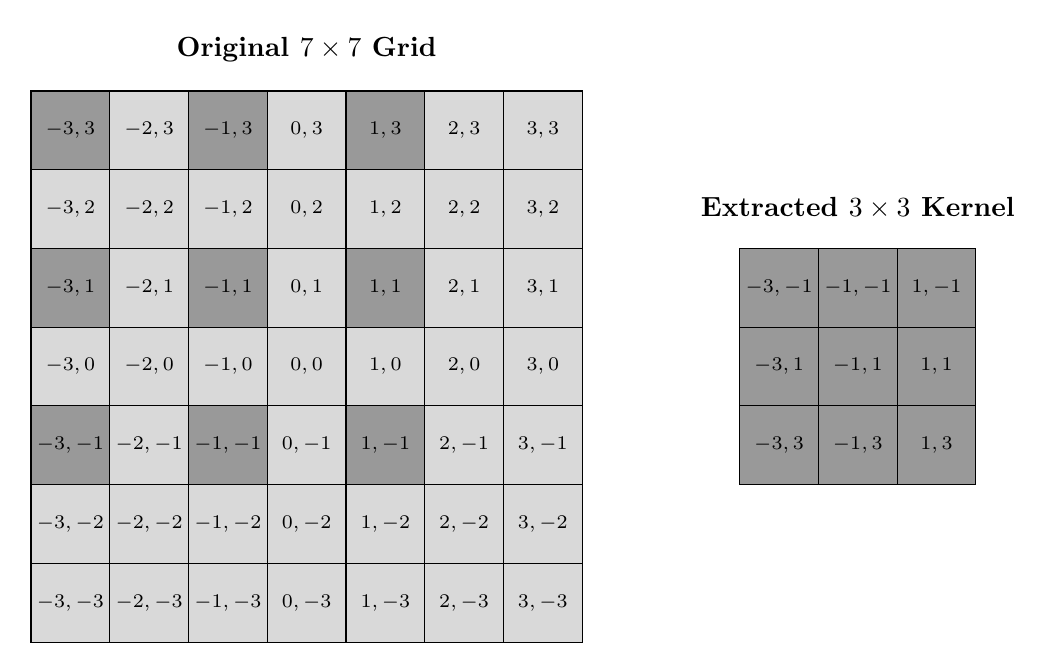
\begin{tikzpicture}
    \foreach \x in {-3,-2,-1,0,1,2,3} {
        \foreach \y in {-3,-2,-1,0,1,2,3} {
            \fill[gray!30] (\x, \y) rectangle (\x+1, \y+1);
            \draw[black] (\x, \y) rectangle (\x+1, \y+1);
        }
    }

    \fill[gray!80] (-3, 3) rectangle (-2, 4);
    \fill[gray!80] (-1, 3) rectangle (0, 4);
    \fill[gray!80] (1, 3) rectangle (2, 4);
    \fill[gray!80] (-3, 1) rectangle (-2, 2);
    \fill[gray!80] (-1, 1) rectangle (0, 2);
    \fill[gray!80] (1, 1) rectangle (2, 2);
    \fill[gray!80] (-3, -1) rectangle (-2, 0);
    \fill[gray!80] (-1, -1) rectangle (0, 0);
    \fill[gray!80] (1, -1) rectangle (2, 0);
    \draw[black] (-3, 3) rectangle (-2, 4);
    \draw[black] (-1, 3) rectangle (0, 4);
    \draw[black] (1, 3) rectangle (2, 4);
    \draw[black] (-3, 1) rectangle (-2, 2);
    \draw[black] (-1, 1) rectangle (0, 2);
    \draw[black] (1, 1) rectangle (2, 2);
    \draw[black] (-3, -1) rectangle (-2, 0);
    \draw[black] (-1, -1) rectangle (0, 0);
    \draw[black] (1, -1) rectangle (2, 0);

    \foreach \x in {-3,-2,-1,0,1,2,3} {
        \foreach \y in {-3,-2,-1,0,1,2,3} {
            \node[font=\scriptsize] at (\x+0.5, \y+0.5) {\scriptsize $\x,\y$};
        }
    }

    \foreach \i [count=\ix from -1] in {-3,-1,1} {
        \foreach \j [count=\jx from -1] in {3,1,-1} {
            \fill[gray!80] (7+\ix, \jx) rectangle (8+\ix, \jx+1);
            \draw[black] (7+\ix, \jx) rectangle (8+\ix, \jx+1);
            \node[font=\scriptsize] at (7.5+\ix, \jx+0.5) {\scriptsize $\i,\j$};
        }
    }

    \node[above] at (0.5, 4.25) {\textbf{Original $7 \times 7$ Grid}};
    \node[above] at (7.5, 2.25) {\textbf{Extracted $3 \times 3$ Kernel}};
\end{tikzpicture}

\caption[Dilated convolution.]{Dilated convolution with kernel size $k = 3$ and dilation rate $d = 2$, illustrated on the $(-1, 1)$ point on a $7 \times 7$ grid.}
\end{figure}

Dilated convolutional layers increase the receptive field of the network exponentially with linear parameter accretion. 

While the idea can be traced back to wavelet decompositions from 1989 \cite{Holschneider1989}, the rediscovery of the method in the machine learning field can be attributed to Chen et al. \cite{Chen2015}.

\subsection{Temporal Convolutional Network}

Temporal Convolutional Network (TCN), introduced by \cite{Colin2016}, leverage the idea of dilated convolutions, to cover varied regions of data in a hierarchical way. The network consists of layers of dilated convolutions, where the dilation rate increases exponentially (e.g., $d = 1, 2, 4, \dots$) across layers.

For sequential or time-series data, this structure efficiently captures both short- and long-term dependencies. Unlike recurrent networks, TCNs process data in parallel, making them computationally efficient.

Compared to recurrent neural networks, TCNs offer several advantages:
\begin{itemize}
	\item \textbf{Parallel Computation}: TCNs allow parallel processing of sequences, unlike recurrent networks where computation is sequential and each state depends on the previous one. This significantly reduces training time.
	\item \textbf{Long-Term Dependency Modeling}: TCNs achieve flexible receptive fields through dilated convolutions, enabling the direct control of dependency range without architectural adjustments.
	\item \textbf{Stability}: Convolutional networks, including TCNs, generally exhibit stable training dynamics. Recurrent networks, on the other hand, are prone to issues such as vanishing or exploding gradients, although gated mechanisms like GRUs mitigate some of these challenges. \end{itemize}

In many cases, these advantages come without sacrificing performance, as we demonstrate in subsequent sections. We evaluate TCNs on various transcription subtasks and provide details about the model structure.

\subsection{Model Architecture}

Since musical features are not spatial, the convolutions are one-dimensional. For our experiments, we used a TCN variant with a kernel size of $9$ and dilation rates of $1$, $2$, and $4$. The receptive field $r$ for $L$ layers can be calculated as follows: \[r = 1 + \sum_{i=1}\left(k_i - 1\right)\cdot d_i\] where $k_i$ and $d_i$ denote the kernel size and dilation rate, respectively, at the $i$-th layer. For three layers, the receptive field is $r_3 = 57$. See Figure \ref{temporal_convolutional_network} for an illustration of the architecture.

\begin{figure}[ht!]
\centering
\begin{tikzpicture}
    \tikzset{layer1/.style={fill=gray!10, draw=gray, thick, text centered}}
    \tikzset{layer2/.style={fill=gray!30, draw=gray, thick, text centered}}
    \tikzset{operation/.style={draw, circle, thick, minimum size=0.75cm}}
    \tikzset{arrowstyle/.style={-{Latex[length=3mm]}}}

    \fill[fill=gray!50, fill opacity=0.5, draw=gray, thick, line width=2pt] (0.0, -2.0) rectangle (12.0, 7.0);
    \fill[fill=white!50, fill opacity=1.0, draw=black, thick, line width=1pt] (0.5, 0.0) rectangle (10.5, 6.5);
    \fill[fill=white!50, fill opacity=1.0, draw=black, thick, line width=1pt] (1.0, -0.5) rectangle (11.0, 6.0);
    \fill[fill=white!50, fill opacity=1.0, draw=black, thick, line width=1pt] (1.5, -1.0) rectangle (11.5, 5.5);

    \draw (6.5, 9.00) node (note_sequence) {Note sequence};
    \draw (6.5, 8.00) node[layer1] (embedding) {Linear};
    \draw (4.0, 4.50) node[layer1] (layerA1) {Dilated Convolutional};
    \draw (4.0, 3.50) node[layer1] (layerA2) {ReLU};
    \draw (4.0, 2.50) node[layer1] (layerA3) {Dropout};
    \draw (4.0, 1.50) node[layer1] (layerA4) {Dilated Convolutional};
    \draw (6.5, 0.75) node[operation] (add) {$+$};
    \draw (6.5, -0.50) node[layer2] (layerA5) {Layer Normalization};
    \draw[anchor=south, inner sep=2pt] (6.5, -2.0) node (outputA) {To the next convolutional layer};

    \draw (6.5, -3.00) node[layer1] (output) {Linear};

    \node[anchor=south west, inner sep=2pt] at (0.2, -1.8) {TCNBlock};

    \node[anchor=north west, inner sep=2pt] at (1.55, 5.45) {\small{9, 1, 256}};
    \node[anchor=north west, inner sep=2pt] at (1.05, 5.95) {\small{9, 2, 256}};
    \node[anchor=north west, inner sep=2pt] at (0.55, 6.45) {\small{9, 4, 256}};
    \node[anchor=north west, inner sep=2pt] at (0.05, 6.95) {\small{kernel size, dilation, hidden size}};

    \draw[arrowstyle] (note_sequence.south) to (embedding.north);
    \draw[arrowstyle] (embedding.south) -| ++(0.0, -2.5) -| (layerA1.north);
    \draw[arrowstyle] (embedding.south) -| ++(0.0, -2.5) -| ++(2.5, 0.0) |- (add.east);
    \draw[arrowstyle] (layerA1.south) to (layerA2.north);
    \draw[arrowstyle] (layerA2.south) to (layerA3.north);
    \draw[arrowstyle] (layerA3.south) to (layerA4.north);
    \draw[arrowstyle] (layerA4.south) |- (add.west);
    \draw[arrowstyle] (add.south) to (layerA5.north);
    \draw[arrowstyle] (layerA5.south) to (outputA.north);
    \draw[arrowstyle] (outputA.south) to (output.north);
\end{tikzpicture}

\caption[The Temporal Convolutional Block.]{The Temporal Convolutional Block.}
\label{temporal_convolutional_network}
\end{figure}

We tested two model variants, with $128$ and $256$ filters per convolutional layer. The training and evaluation procedures followed the same setup as the baseline models.

\subsection{Results}

Experiments with TCNs showed that these networks achieved comparable or superior performance for certain transcription subtasks, while requiring fewer parameters and training faster compared to recurrent networks.

We use standard abbreviations for the metrics: \emph{acc}, \emph{prec}, \emph{rec} and $F$ for accuracy, precision, recall and $F_1$ score, respectively.

\subsubsection{Beat Model}

The beat quantization task was less suited to the TCN architecture. While the larger TCN variant performed close to the baseline, the original model consistently outperformed both TCN variants.

\begin{table}[ht!]
\centering
\begin{tabular}{cc|ccc}
    \multicolumn{2}{c|}{\textbf{Model}} & \textbf{Original} & \textbf{TCN 128} & \textbf{TCN 256} \\
    \multicolumn{2}{c|}{\textbf{Parameters}} & 27.5 M & 7.6 M & 10.9 M \\\hline
    \multirow{4}{*}{Beats}     & Accuracy    & $\mathbf{0.880}$ & $ $ & $0.848$          \\
    & Precision   & $\mathbf{0.879}$ & $ $ & $0.832$          \\
    & Recall      & $\mathbf{0.873}$ & $ $ & $0.831$          \\
    & $F_1$ score & $\mathbf{0.864}$ & $ $ & $0.819$          \\\hline
    \multirow{4}{*}{Downbeats} & Accuracy    & $\mathbf{0.853}$ & $ $ & $\mathbf{0.867}$ \\
    & Precision   & $0.622$          & $ $ & $0.660$ \\
    & Recall      & $\mathbf{0.467}$ & $ $ & $0.568$          \\
    & $F_1$ score & $\mathbf{0.508}$ & $ $ & $0.577$          \\\hline
    \multirow{4}{*}{Beats}     & Accuracy    & $\mathbf{0.869}$ & $0.823$ & $0.851$          \\
    & Precision   & $\mathbf{0.859}$ & $0.795$ & $0.842$          \\
    & Recall      & $\mathbf{0.884}$ & $0.848$ & $0.847$          \\
    & $F_1$ score & $\mathbf{0.859}$ & $0.802$ & $0.831$          \\\hline
    \multirow{4}{*}{Downbeats} & Accuracy    & $\mathbf{0.860}$ & $0.854$ & $\mathbf{0.860}$ \\
    & Precision   & $0.665$          & $0.640$ & $\mathbf{0.704}$ \\
    & Recall      & $\mathbf{0.486}$ & $0.453$ & $0.406$          \\
    & $F_1$ score & $\mathbf{0.545}$ & $0.513$ & $0.494$          \\\hline
    \multicolumn{2}{c|}{Meter} & $\mathbf{0.579}$ & $0.537$ & $0.576$ \\
\end{tabular}

\caption[Temporal Convolutional Network results for the beat model.]{Temporal Convolutional Network results for the beat model.}
\label{beat_tcn}
\end{table}

Adding more layers or increasing the receptive field worsened model performance, indicating that the architecture may require further tuning for this task. 

The dynamic programming algorithm for out-of-note beat prediction has been left intact.

\subsubsection{Hand Part Model}

The TCN-based hand part model achieved results comparable to the baseline while benefiting from a significantly smaller and faster architecture. This suggests that recurrent networks are not strictly necessary for the hand part assignment task.

\begin{table}[ht!]
\centering
\begin{tabular}{c|ccc}
    \textbf{Model}      & \textbf{Original} & \textbf{TCN 128} & \textbf{TCN 256} \\
    \textbf{Parameters} & 10.5 M           & 954 K            & 3.7 M            \\\hline
    Accuracy            & $\mathbf{0.956}$ & $0.917$          & $0.919$          \\
    Precision           & $0.851$          & $\mathbf{0.908}$ & $\mathbf{0.908}$ \\
    Recall              & $0.848$          & $0.865$          & $\mathbf{0.872}$ \\
    $F_1$ score         & $0.842$          & $0.885$          & $\mathbf{0.888}$ \\
    Voice separation    & $\mathbf{0.820}$ & $0.805$          & $0.806$          \\
\end{tabular}
\caption[Temporal Convolutional Network results for the hand part model.]{Temporal Convolutional Network results for the hand part model.}
\label{hand_part_tcn}
\end{table}

\subsubsection{Key Signature Model}

The TCN-based key signature model struggled with rarer key signatures, resulting in a noticeable gap between macro and weighted metrics. Variants with more layers didn't improve the quality of the model.

\begin{table}[ht!]
\centering
\begin{tabular}{cc|ccc}
    \multicolumn{2}{c|}{\textbf{Model}} & \textbf{Original} & \textbf{TCN 128} & \textbf{TCN 256} \\
    \multicolumn{2}{c|}{\textbf{Parameters}} & 10.5 M & 955 K & 3.7 M \\\hline
    \multirow{3}{*}{Macro}    & Precision   & $\mathbf{0.812}$ & $0.307$          & $0.351$ \\
    & Recall      & $\mathbf{0.789}$ & $0.239$          & $0.284$ \\
    & $F_1$ score & $\mathbf{0.787}$ & $0.260$          & $0.307$ \\\hline
    \multirow{3}{*}{Weighted} & Precision   & $0.924$          & $\mathbf{0.954}$ & $0.951$ \\
    & Recall      & $\mathbf{0.898}$ & $0.673$          & $0.682$ \\
    & $F_1$ score & $\mathbf{0.896}$ & $0.771$          & $0.777$ \\\hline
    \multicolumn{2}{c|}{Harmony} & $\mathbf{0.972}$ & $0.878$ & $0.834$ \\
\end{tabular}

\caption[Temporal Convolutional Network results for the key signature model.]{Temporal Convolutional Network results for the key signature model.}
\label{key_signature_tcn}
\end{table}

\subsubsection{Time Signature Model}

The TCN-based time signature model significantly outperformed the baseline convolutional network. As observed in earlier experiments, time signature estimation does not impact the MV2H metric.

\begin{table}[ht!]
\centering
\begin{tabular}{c|ccc}
    \textbf{Model}      & \textbf{Original} & \textbf{TCN 128} & \textbf{TCN 256} \\
    \textbf{Parameters} & 676 K             & 954 K            & 3.7 M            \\\hline
    Accuracy            & $0.560$           & $\mathbf{0.612}$ & $0.575$          \\
    Precision           & $\mathbf{0.315}$  & $0.280$          & $0.261$          \\
    Recall              & $0.230$           & $\mathbf{0.236}$ & $0.249$          \\
    $F_1$ score         & $\mathbf{0.258}$  & $0.248$          & $0.253$          \\\hline
    Accuracy            & $0.552$           & $0.655$          & $\mathbf{0.793}$ \\
    Precision           & $0.444$           & $0.625$          & $\mathbf{0.750}$ \\
    Recall              & $0.333$           & $0.417$          & $\mathbf{0.750}$ \\
    $F_1$ score         & $0.381$           & $0.500$          & $\mathbf{0.750}$ \\
\end{tabular}
\caption[Temporal Convolutional Network results for the time signature model.]{Temporal Convolutional Network results for the time signature model.}
\label{time_signature_tcn}
\end{table}

\section{Dynamics}

In a musical score, dynamics indicate the intensity or volume with which notes should be played. To enhance the transcription capabilities of the model, we introduced a new submodule for transcribing dynamics. This submodule classifies notes into one of ten dynamic levels, ranging from $\lilyDynamics{pppp}$ (very soft) to $\lilyDynamics{ffff}$ (very loud). Several simplifications were made to address common challenges in interpreting dynamics:
\begin{itemize}
	\item Gradual dynamic changes such as \emph{crescendo} and \emph{diminuendo} were excluded.
	\item Accents on individual notes (marked as $>$) were not considered.
	\item Dynamics were assumed to apply uniformly to both hands, disallowing independent dynamics for left and right hands.
	\end{itemize}

As in standard musical practice, dynamic markings are displayed only when there is a change. If no marking is explicitly given, \emph{mezzo-forte} is assumed as the default level. The dynamics model operates independently of the other transcription submodules.

\subsection{Architecture}

The architecture of the dynamics model follows the modular design of other submodules. It mirrors the structure of the key signature model, comprising convolutional layers, a GRU block, and a final linear layer with 10 output categories corresponding to the dynamics levels.

The extended architecture of the model, including the dynamics module, is shown in Figure \ref{model_architecture_extended}. The modularity of the model enables the dynamics block to be replaced with alternative architectures, such as Transformer or TCN-based blocks.

\begin{figure}[!ht]
\centering
\begin{tikzpicture}
    \tikzset{sequence/.style={thick, text centered, align=center}}
    \tikzset{convblock/.style={fill=gray!20, draw=gray, thick, text centered}}
    \tikzset{grublock/.style={fill=gray!30, draw=gray, thick, text centered}}
    \tikzset{linear/.style={fill=gray!10, draw=gray, thick, text centered}}
    \tikzset{output/.style={thick, anchor=west, align=left}}
    \tikzset{arrowstyle/.style={-{Latex[length=3mm]}}}
    \draw (-3.5, 0.5) node[sequence] (sequence) {note\\ sequence};

    \draw (-1.75, 5) node (joint1) {};
    \draw (-1.75, 3) node (joint2) {};
    \draw (-1.75, 2) node (joint3) {};
    \draw (-1.75, 0.5) node (joint4) {};
    \draw (-1.75, -1) node (joint5) {};
    \draw (-1.75, -2) node (joint6) {};
    \draw (-1.75, -3) node (joint7) {};

    \draw (1.5, 3) node (concatenation) {$\boldsymbol{\oplus}$};
    \draw (1.5, 3.5) node (concatleftjoint1) {};
    \draw (1.5, 2.5) node (concatleftjoint2) {};
    \draw (7.25, 3.5) node (concatrightjoint1) {};
    \draw (7.25, 2.5) node (concatrightjoint2) {};
    \draw (7.25, 2) node (concatstart1) {};
    \draw (7.25, 4) node (concatstart2) {};

    \draw (0, 5) node[convblock] (convblock1) {ConvBlock};
    \draw (0, 3) node[convblock] (convblock2) {ConvBlock};
    \draw (0, 2) node[convblock] (convblock3) {ConvBlock};
    \draw (0, 0.5) node[convblock] (convblock4) {ConvBlock};
    \draw (0, -1) node[convblock] (convblock5) {ConvBlock};
    \draw (0, -2) node[convblock] (convblock6) {ConvBlock};
    \draw (0, -3) node[convblock] (convblock7) {ConvBlock};

    \draw (3, 6) node[grublock] (grublock1) {GRUBlock};
    \draw (3, 5) node[grublock] (grublock2) {GRUBlock};
    \draw (3, 4) node[grublock] (grublock3) {GRUBlock};
    \draw (3, 3) node[grublock] (grublock4) {GRUBlock};
    \draw (3, 2) node[grublock] (grublock5) {GRUBlock};
    \draw (3, 0.5) node[grublock] (grublock6) {GRUBlock};
    \draw (3, -1) node[grublock] (grublock7) {GRUBlock};
    \draw (3, -2) node[grublock] (grublock8) {GRUBlock};
    \draw (3, -3) node[grublock] (grublock9) {GRUBlock};

    \draw (6, 6) node[linear] (linear1) {Linear (200)};
    \draw (6, 5) node[linear] (linear2) {Linear (1)};
    \draw (6, 4) node[linear] (linear3) {Linear (1)};
    \draw (6, 3) node[linear] (linear4) {Linear (24)};
    \draw (6, 2) node[linear] (linear5) {Linear (96)};
    \draw (6, 1) node[linear] (linear6) {Linear (5)};
    \draw (6, 0) node[linear] (linear7) {Linear (4)};
    \draw (6, -1) node[linear] (linear8) {Linear (12)};
    \draw (6, -2) node[linear] (linear9) {Linear (1)};
    \draw (6, -3) node[linear] (linear10) {Linear (10)};

    \draw (7.75, 6) node[output] (output1) {tempo};
    \draw (7.75, 5) node[output] (output2) {downbeats};
    \draw (7.75, 4) node[output] (output3) {beats};
    \draw (7.75, 3) node[output] (output4) {musical onsets};
    \draw (7.75, 2) node[output] (output5) {note values};
    \draw (7.75, 1) node[output] (output6) {time signature\\  numerators};
    \draw (7.75, 0) node[output] (output7) {time signature\\  denominators};
    \draw (7.75, -1) node[output] (output8) {key signature};
    \draw (7.75, -2) node[output] (output9) {hand parts};
    \draw (7.75, -3) node[output] (output10) {dynamics};

    \draw (sequence) to (joint4.center);
    \draw (joint1.center) to (joint7.center);
    \draw[arrowstyle] (joint1.center) to (convblock1);
    \draw[arrowstyle] (joint2.center) to (convblock2);
    \draw[arrowstyle] (joint3.center) to (convblock3);
    \draw[arrowstyle] (joint4.center) to (convblock4);
    \draw[arrowstyle] (joint5.center) to (convblock5);
    \draw[arrowstyle] (joint6.center) to (convblock6);
    \draw[arrowstyle] (joint7.center) to (convblock7);

    \draw[arrowstyle] (convblock1.east) to (grublock1.west);
    \draw[arrowstyle] (convblock1.east) to (grublock2.west);
    \draw[arrowstyle] (convblock1.east) to (grublock3.west);
    \draw[arrowstyle] (convblock2.east) to (grublock4.west);
    \draw[arrowstyle] (convblock3.east) to (grublock5.west);
    \draw[arrowstyle] (convblock4.east) to (grublock6.west);
    \draw[arrowstyle] (convblock5.east) to (grublock7.west);
    \draw[arrowstyle] (convblock6.east) to (grublock8.west);
    \draw[arrowstyle] (convblock7.east) to (grublock9.west);

    \draw[arrowstyle] (grublock1.east) to (linear1.west);
    \draw[arrowstyle] (grublock2.east) to (linear2.west);
    \draw[arrowstyle] (grublock3.east) to (linear3.west);
    \draw[arrowstyle] (grublock4.east) to (linear4.west);
    \draw[arrowstyle] (grublock5.east) to (linear5.west);
    \draw[arrowstyle] (grublock6.east) to (linear6.west);
    \draw[arrowstyle] (grublock6.east) to (linear7.west);
    \draw[arrowstyle] (grublock7.east) to (linear8.west);
    \draw[arrowstyle] (grublock8.east) to (linear9.west);
    \draw[arrowstyle] (grublock9.east) to (linear10.west);

    \draw[arrowstyle] (linear1.east) to (output1.west);
    \draw[arrowstyle] (linear2.east) to (output2.west);
    \draw[arrowstyle] (linear3.east) to (output3.west);
    \draw[arrowstyle] (linear4.east) to (output4.west);
    \draw[arrowstyle] (linear5.east) to (output5.west);
    \draw[arrowstyle] (linear6.east) to (output6.west);
    \draw[arrowstyle] (linear7.east) to (output7.west);
    \draw[arrowstyle] (linear8.east) to (output8.west);
    \draw[arrowstyle] (linear9.east) to (output9.west);
    \draw[arrowstyle] (linear10.east) to (output10.west);

    \draw[arrowstyle, dashed] (concatleftjoint1.center) to (concatenation.center);
    \draw[arrowstyle] (concatleftjoint2.center) to (concatenation.center);
    \draw[dashed] (concatleftjoint1.center) to (concatrightjoint1.center);
    \draw (concatleftjoint2.center) to (concatrightjoint2.center);
    \draw (concatstart1.center) to (concatrightjoint2.center);
    \draw[dashed] (concatstart2.center) to (concatrightjoint1.center);

    \draw (3.5, -4) node[output] (legendsymbol1) {$\boldsymbol{\oplus}$};
    \draw (3, -4.75) node[output] (legendsymbolstart) {};
    \draw (4.5, -4.75) node[output] (legendsymbolend) {};
    \draw (5, -4) node[output] (legend1) {concatenation};
    \draw (5, -4.75) node[output] (legend2) {disable backpropagation during training};
    \draw[arrowstyle, dashed] (legendsymbolstart.center) to (legendsymbolend.center);
\end{tikzpicture}
 \caption[Extended model architecture with dynamics module.]{The extended architecture of the model, incorporating the \emph{dynamics} module. Note that the quantization model is not shown, as it does not directly contribute to the final MIDI score generation.}
\label{model_architecture_extended}
\end{figure}

\subsection{Challenges}

Two major challenges arose during the development of the dynamics model:
\begin{itemize} \item No direct dynamics annotations exist in any of the datasets considered. \item The interpretation of dynamics in musical performances is subjective and thus varies considerably. \end{itemize}

\subsubsection{Dynamics Data}

The ACPAS dataset does not contain any direct information about dynamics. Neither the MIDI files nor the annotations provide this data. Among the three datasets used, only the ASAP dataset includes dynamics annotations, but only for the ground truth score in the MusicXML format.

For the performance MIDI files in the ASAP dataset, dynamics annotations were recovered through an imperfect automation process. Table \ref{annotations_dynamics} presents an example of the augmented annotation structure.

\begin{table}[ht!]
\centering
\begin{tabular}{ccc}
    Timestamp  & Timestamp  & Annotation          \\\hline
    $2.845313$ & $2.845313$ & db, $6/8$, $2$, $f$ \\
    $3.446876$ & $3.446876$ & b                   \\
    $3.858854$ & $3.858854$ & db                  \\
    $4.218229$ & $4.218229$ & b
\end{tabular}

\caption[Dynamics TSV annotations for the ASAP dataset.]{An example of augmented dynamics annotations in the ASAP dataset, showing a starting \emph{forte} dynamics marking encoded as $f$.}
\label{annotations_dynamics}
\end{table}

Additionally, certain musical pieces, such as those written for the harpsichord or organ (e.g., some of Bach's fugues), lack dynamic markings, limiting the dataset even more.

\subsubsection{Matching Algorithm}

The matching algorithm parses the original ground truth MusicXML score to extract dynamics annotation positions aligned to corresponding note blocks.

MIDI performance files use absolute time in seconds, while scores are in beats, so direct comparison is not possible. To overcome this, we employed a basic matching algorithm that relies on the ratio of already played notes to the total number of notes. Deviations are allowed to account for missing or extra notes.

Chords with a dynamics annotation from the score are matched to chords with identical notes and corresponding positions in the original performance. Any unmatched or misaligned chords are discarded.

While more sophisticated algorithms (e.g., Dynamic Time Warping) could be used, we opted for simplicity. We believe that high-quality dynamics annotations are essential for building a reliable dynamics model, and even more advanced matching algorithms are unlikely to resolve the core issue of data quality. The current solution is a preliminary step toward incorporating a richer vocabulary for musical scores.

\subsection{Subjectivity of Dynamics Markings}

A significant challenge in modeling dynamics is the inherent subjectivity of dynamics annotations. The interpretation of dynamics depends on various factors, including the instrument on which the music is performed, the era and genre of the music, and the performing style of the musician.

This variability leads to considerable differences in expected outcomes, as the relationship between the score and the performance is far from exact.

\subsection{Evaluation}

The model was trained using the standard negative log-likelihood loss, similar to the approach used for the key signature model. We evaluated the model using the standard set of multiclass classification metrics, with the macro $F_1$ score as the final evaluation metric, consistent with the evaluation scheme for the key signature model.

To avoid penalizing misclassifications between similar dynamic classes (e.g., distinguishing $\lilyDynamics{f}$ from $\lilyDynamics{ff}$), one could apply a standard distance metric between labels, where $0$ represents the softest dynamics, $\lilyDynamics{pppp}$, and $1$ represents the loudest, $\lilyDynamics{ffff}$. However, we followed the same setup as the key signature model for simplicity.

\subsubsection{MV2HD}

Since dynamics can be evaluated independently of other features, assuming they are correctly aligned with the note stream, we propose an enhancement to the MV2H metric, called \textbf{MV2HD}, where D stands for dynamics. The dynamics submetric is simply the $F_1$ score for correctly aligned notes, and the total metric is calculated as: \[\textrm{MV2HD} = \tfrac{5}{6}\textrm{MV2HD} + \tfrac{1}{6}F_1\] Here, $F_1$ is the dynamics submetric score. Since the $F_1$ score lies in the interval $[0, 1]$, the MV2HD metric is bounded between $0$ and $1$. The weight of $\tfrac{1}{6}$ for dynamics is debatable, as dynamics do not play the same role as, for example, meter alignment. However, this weight was chosen for symmetry in the overall metric.

Because dynamics are independent of other features, the MV2HD metric still adheres to the principle of disjoint penalties.

Currently, the MV2HD metric is a theoretical proposal and would require implementation in the Java code provided by McLeod et al. \cite{McLeod2019}.

\subsubsection{Results}

\missing